\documentclass[aspectratio=169, 14pt]{beamer}
\usepackage[utf8]{inputenc}
\usepackage[english]{babel}
\usepackage{tipa}
\newcommand*{\codefont}{\fontfamily{Comic Sans MS}\selectfont}
\usepackage{graphicx}
\usepackage{transparent}
\usepackage[ruled, lined, linesnumbered, commentsnumbered]{algorithm2e}
\usepackage{tikz}
\usetikzlibrary{calc,shadows.blur}
\usetikzlibrary{matrix,backgrounds}
\usepackage{minted}
\usepackage{csquotes}
\usepackage{outlines}
\usepackage{fontawesome5}
\usepackage{booktabs}
\usepackage{hyperref}
\hypersetup{
    colorlinks=true,
    linkcolor=blue,
    filecolor=magenta,      
    urlcolor=cyan,
    }
\urlstyle{same}
\usetheme{metropolis}
\metroset{block=fill}
\usecolortheme{default}
\definecolor{darkmidnightblue}{rgb}{0.0, 0.2, 0.4}
\definecolor{LightGray}{gray}{0.9}


%------------------------------------------------------------
%This block of code defines the information to appear in the
%Title page
\title[Data Structures] %optional
{Data Structures}

\subtitle{Built-in Data Structures}

\author[CHEN Zhongpu] % (optional)
{CHEN Zhongpu}

\institute[] % (optional)
{
  School of Computing and Artificial Intelligence \\
  \href{mailto:zpchen@swufe.edu.cn}{zpchen@swufe.edu.cn}
}

\date[] % (optional)
{SWUFE, Fall 2022}

%End of title page configuration block
%------------------------------------------------------------


%------------------------------------------------------------
%The next block of commands puts the table of contents at the 
%beginning of each section and highlights the current section:

% \AtBeginSection[]
% {
%   \begin{frame}
%     \frametitle{Table of Contents}
%     \tableofcontents[currentsection]
%   \end{frame}
% }
%------------------------------------------------------------


\begin{document}

%The next statement creates the title page.
\frame{\titlepage}

%---------------------------------------------------------
%This block of code is for the table of contents after
%the title page
% \begin{frame}
% \frametitle{Table of Contents}
% \tableofcontents
% \end{frame}
%--------------------------------------------------------
\begin{frame}
    \Large $$Data\ Structure + Algorithm = Program$$
\end{frame}

{
    % \usebackgroundtemplate{\transparent{0.3}{\begin{picture}
    %     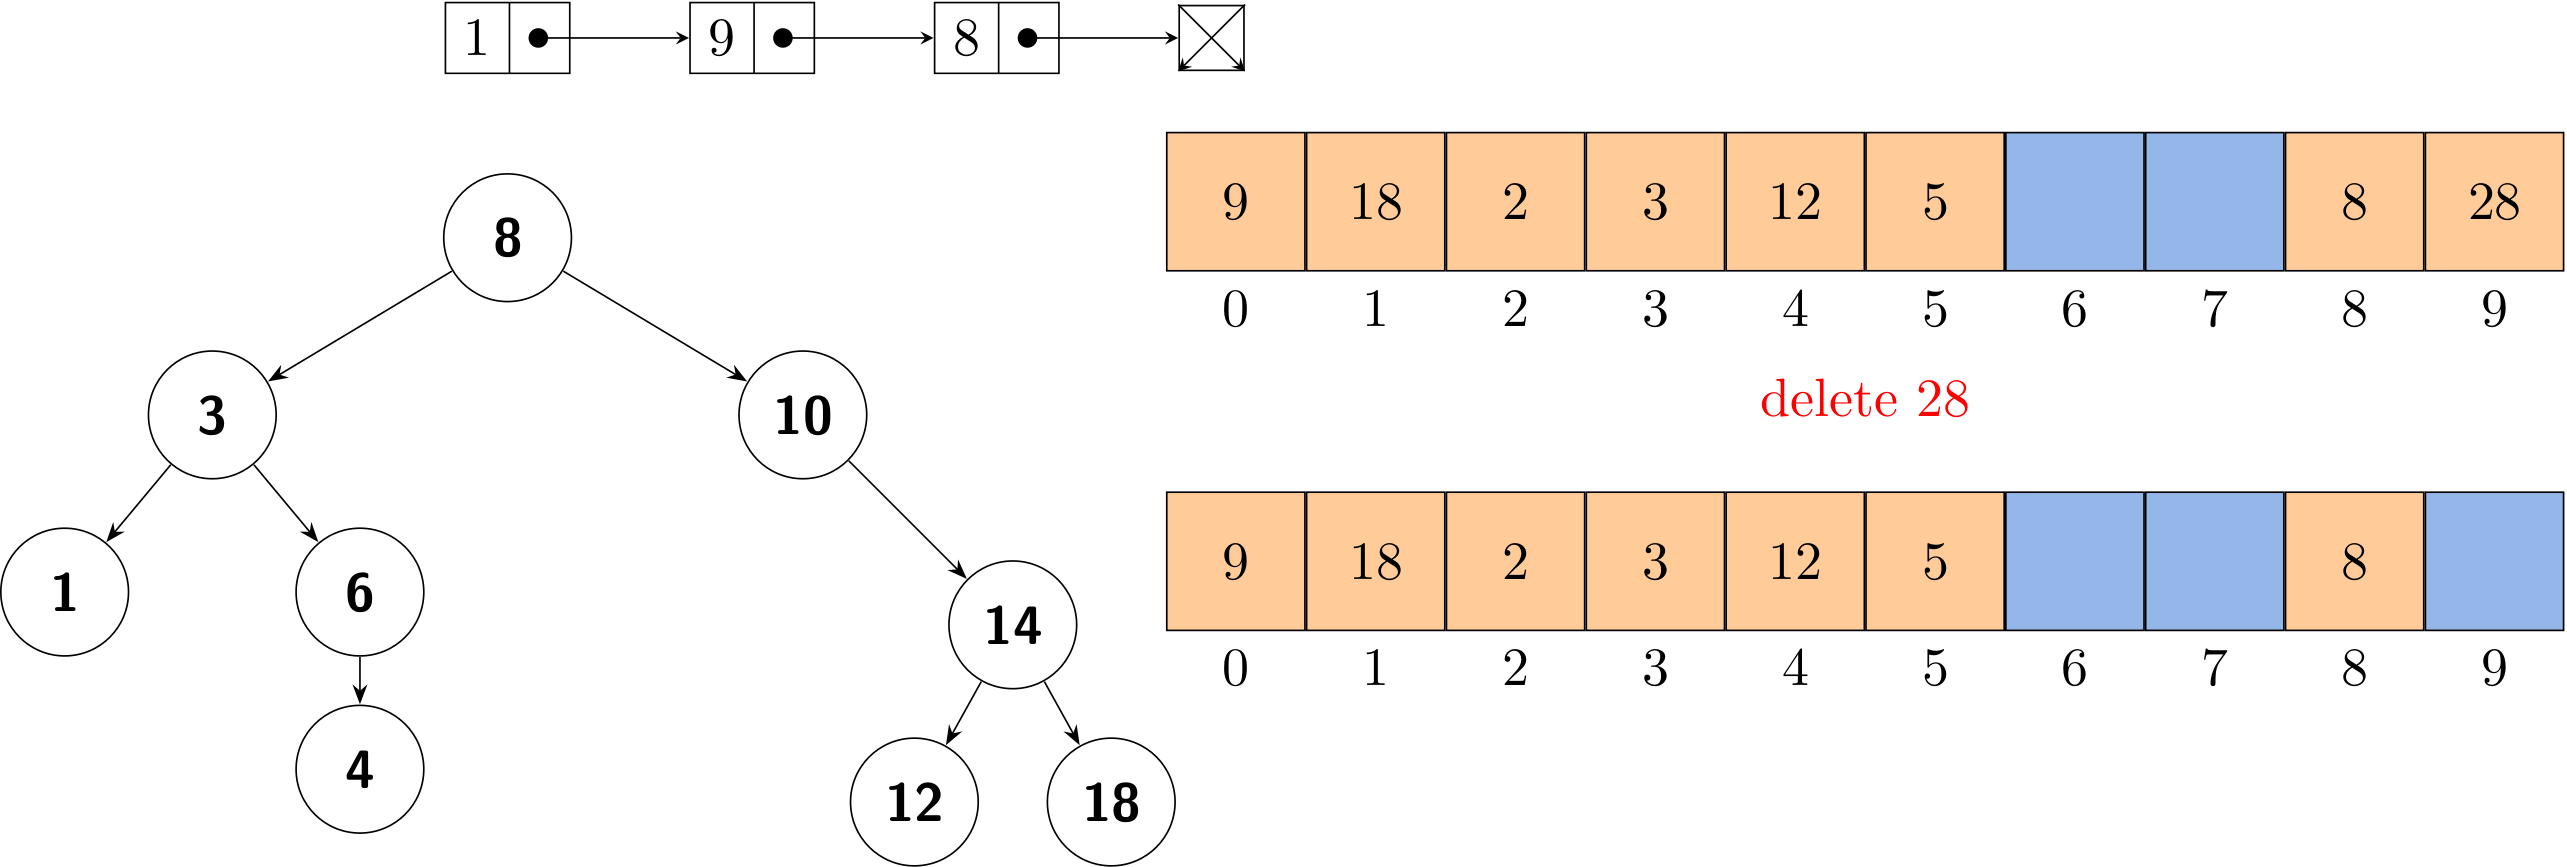
\includegraphics[height=0.7\paperheight]{cover}
    % \end{picture}    
    % }}
\usebackgroundtemplate{
  \tikz[overlay,remember picture] 
  \node[opacity=0.3, at=(current page.south east),anchor=south east, yshift=2cm,xshift=4cm] {
    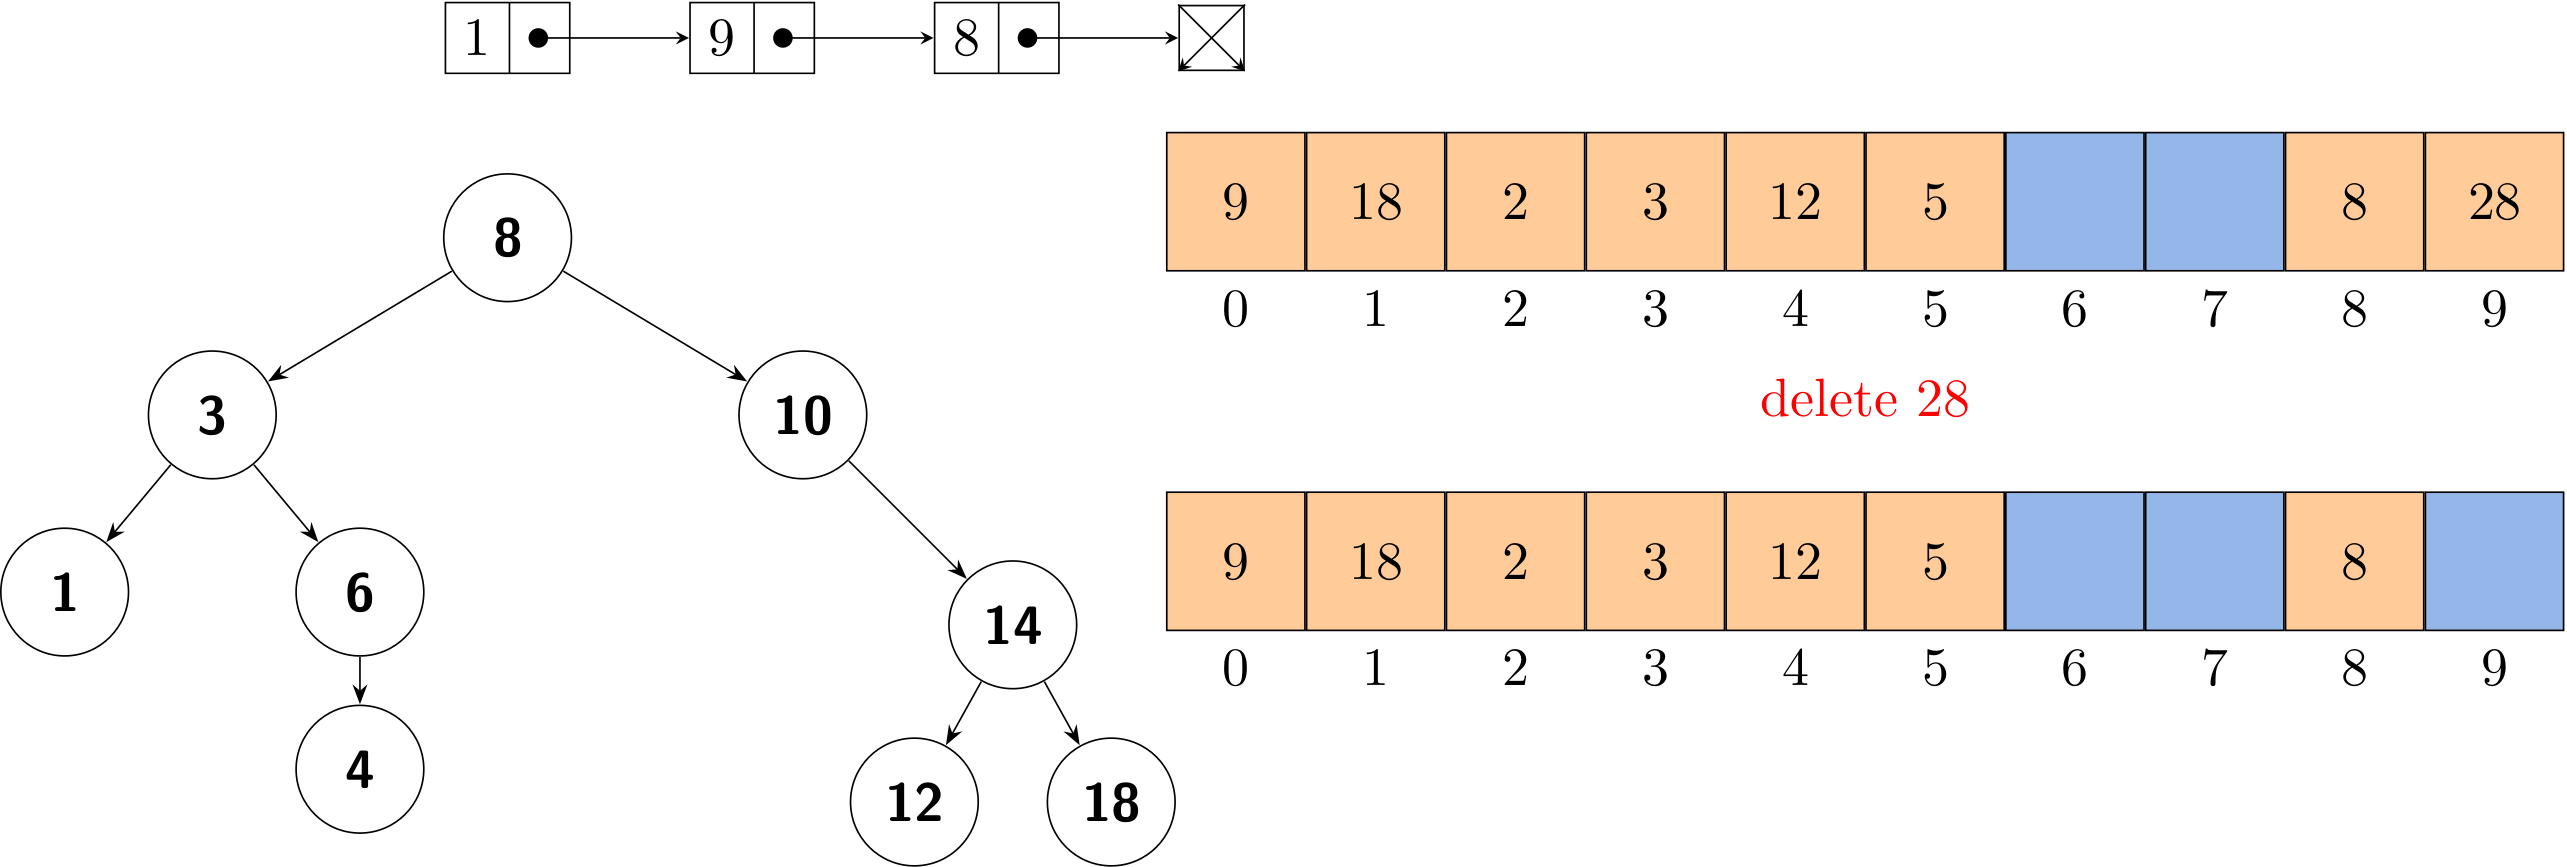
\includegraphics[height=0.6\paperheight]{cover}};
}
    \begin{frame}
        \section{\textcolor{darkmidnightblue}{1. Java Built-in Data Structures}}
    \end{frame}

}

\begin{frame}{Containter}
    \begin{quote}
        A \alert{collection} — sometimes called a \alert{container} — is simply an object that groups multiple elements into a single unit.
    \end{quote}

    \begin{itemize}
        \item \textbf{Library}: a group of books
        \item \textbf{School}: a group of students
        \item \textbf{E-commerce}: a group of shopping cart items
        \item \textbf{Airline}: a group of tickets 
        \item \dots
    \end{itemize}
\end{frame}

\begin{frame}[fragile]
    \frametitle{1.1 Array}
    \begin{quote}
        An \alert{array} is a container object that holds a fixed number of values of a single type.
    \end{quote}
    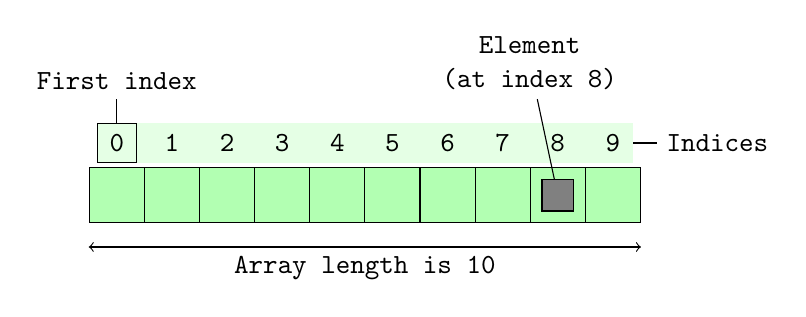
\begin{tikzpicture}[font=\ttfamily,
        array/.style={matrix of nodes,nodes={draw, minimum size=7mm, fill=green!30},column sep=-\pgflinewidth, row sep=0.5mm, nodes in empty cells,
        row 1/.style={nodes={draw=none, fill=none, minimum size=5mm}},
        row 1 column 1/.style={nodes={draw}}}]
        
        \matrix[array] (array) {
        0 & 1 & 2 & 3 & 4 & 5 & 6 & 7 & 8 & 9\\
          &   &   &   &   &   &   &   &   &  \\};
        \node[draw, fill=gray, minimum size=4mm] at (array-2-9) (box) {};
        
        \begin{scope}[on background layer]
        \fill[green!10] (array-1-1.north west) rectangle (array-1-10.south east);
        \end{scope}
        
        \draw[<->]([yshift=-3mm]array-2-1.south west) -- node[below] {Array length is 10} ([yshift=-3mm]array-2-10.south east);
        
        \draw (array-1-1.north)--++(90:3mm) node [above] (first) {First index};
        \draw (array-1-10.east)--++(0:3mm) node [right]{Indices};
        \node [align=center, anchor=south] at (array-2-9.north west|-first.south) (8) {Element\\ (at index 8)};
        \draw (8)--(box);
    \end{tikzpicture}
\end{frame}

\begin{frame}[fragile]
    \begin{columns}
        \column{0.4\textwidth}
        Making an array in a Java program involves three distinct steps:
        \begin{enumerate}
            \item Declare the array name and type.
            \item Create the array.
            \item Initialize the array.
        \end{enumerate}
        \column{0.59\textwidth}
        \begin{minted}
            [
                bgcolor=LightGray
            ]
        {java}
double[] a; // declare
a = new double[N]; // create
for (int i = 0; i < N; i++) {
    a[i] = 3.14; // initialize
}            
        \end{minted}
        \begin{minted}[bgcolor=LightGray]{java}
double[] a = {3.14, 3.15, 3.16};            
        \end{minted}
    \end{columns}
\end{frame}

\begin{frame}[fragile]
        \begin{minted}
            [
                bgcolor=LightGray
            ]
        {java}
        for (int i = 0; i < N; i++) {
            System.out.println(a[i]);
        }        
        \end{minted}
Enhanced \textbf{for} statement (a.k.a., \emph{for-each}).
        \begin{minted}
            [
                bgcolor=LightGray
            ]
        {java}
        for (double d : a) {
            System.out.println(d);
        }      
        \end{minted} 
\end{frame}

\begin{frame}[fragile]
    \frametitle{1.2 ArrayList}
    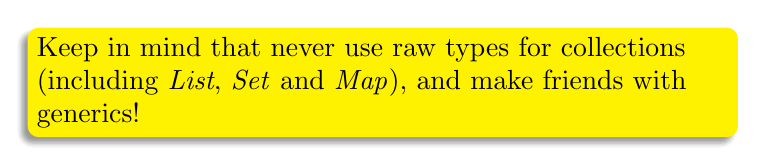
\begin{tikzpicture}
        \node[fill=yellow,blur shadow={shadow xshift=-0.5ex},
        text width=25em,anchor=south west,rounded corners]
        {Keep in mind that never use raw types for collections (including \emph{List}, \emph{Set} and \emph{Map}), and make friends with generics!};
    \end{tikzpicture}
    \begin{minted}
        [
            bgcolor=LightGray
        ]
    {java}
    // generics
    List<String> books = new ArrayList<>(); 
    //  don't do this!
    List fruits = new ArrayList(); 
    \end{minted} 
\end{frame}
\begin{frame}
    Basically, you can regard \alert{List} as a more powerful array, and you are required to know and practice at least those methods:
    \begin{enumerate}
        \item \texttt{add()}
        \item \texttt{addAll()}
        \item clear()
        \item contains()
        \item get()
        \item indexOf()
        \item remove()
        \item size()
        \item toArray()
    \end{enumerate}
\end{frame}

\begin{frame}[fragile]
    \frametitle{Collections}
    \href{https://docs.oracle.com/en/java/javase/11/docs/api/java.base/java/util/Collections.html}{java.util.Collections} provides plenty of handy static methods.

\begin{minted}[bgcolor=LightGray]{java}
List<Integer> list = Arrays.asList(1, 9, 4, 2);
int v = Collections.max(list); 
Collections.sort(list);  
Collections.reverse(list);
\end{minted}
\end{frame}


\begin{frame}
    \frametitle{1.3 HashMap}
    \alert{Map} can be used to represent a mapping between a \emph{key} and a \emph{value}, and we assume that keys are unique.
    \begin{table}
        \caption{Key-value examples}
        \begin{tabular}{lr}
          \toprule
          Key & Value\\
          \midrule
          Name & Age\\
          Country & GDP\\
          ISBN & Price \\
          \bottomrule
        \end{tabular}
    \end{table}
\end{frame}

\begin{frame}[fragile]
    Let's consider a \textbf{shopping cart} which maintains pairs of ISBN (key) and amount (value).

    \begin{minted}[bgcolor=LightGray]{java}
Map<String, Integer> cart = new HashMap<>();

cart.put("7801", 3);
int amount = cart.get("7801");

for (var entry : cart.entrySet()) {
    System.out.println(entry.getKey());
    System.out.println(entry.getValue());
}
    \end{minted}
\end{frame}

\begin{frame}[fragile]
    \frametitle{}
    What if the index/key does not exist?    
    \begin{minted}[bgcolor=LightGray]{java}
List<String> cities = new ArrayList<>();
cities.add("Paris");
cities.add("Shanghai");
String name = cities.get(2);
    \end{minted}

    \begin{minted}[bgcolor=LightGray]{java}
Map<String, Integer> cart = new HashMap<>();
cart.put("7801", 3);
int amount = cart.get("7802");
    \end{minted}  
\end{frame}

\begin{frame}
    You are required to know and practice at least those methods:
    \begin{enumerate}
        \item clear()
        \item containsKey()
        \item entrySet()
        \item get()
        \item getOrDefault()
        \item isEmpty()
        \item keySet()
        \item put()
        \item remove()
        \item size()
        \item values()
    \end{enumerate}
\end{frame}

\begin{frame}[fragile]
    \frametitle{1.4 HashSet}
    \begin{minted}[bgcolor=LightGray]{java}
Set<String> set = new HashSet<>();
set.add("hello");
set.add("world");
System.out.println(set.size()); // 2
set.add("hello");
System.out.println(set.size()); // 2
    \end{minted}      
    \begin{quote}
        \alert{Set} is a collection that contains no duplicate elements. It is essentially a \alert{Map} without the \emph{value}.
    \end{quote}
\end{frame}

\begin{frame}
    You are required to know and practice at least those methods:

\begin{enumerate}
\item add()
\item clear()
\item contains()
\item isEmpty()
\item remove()
\item size()
\end{enumerate}
\end{frame}

{
    % \usebackgroundtemplate{\transparent{0.3}{\begin{picture}
    %     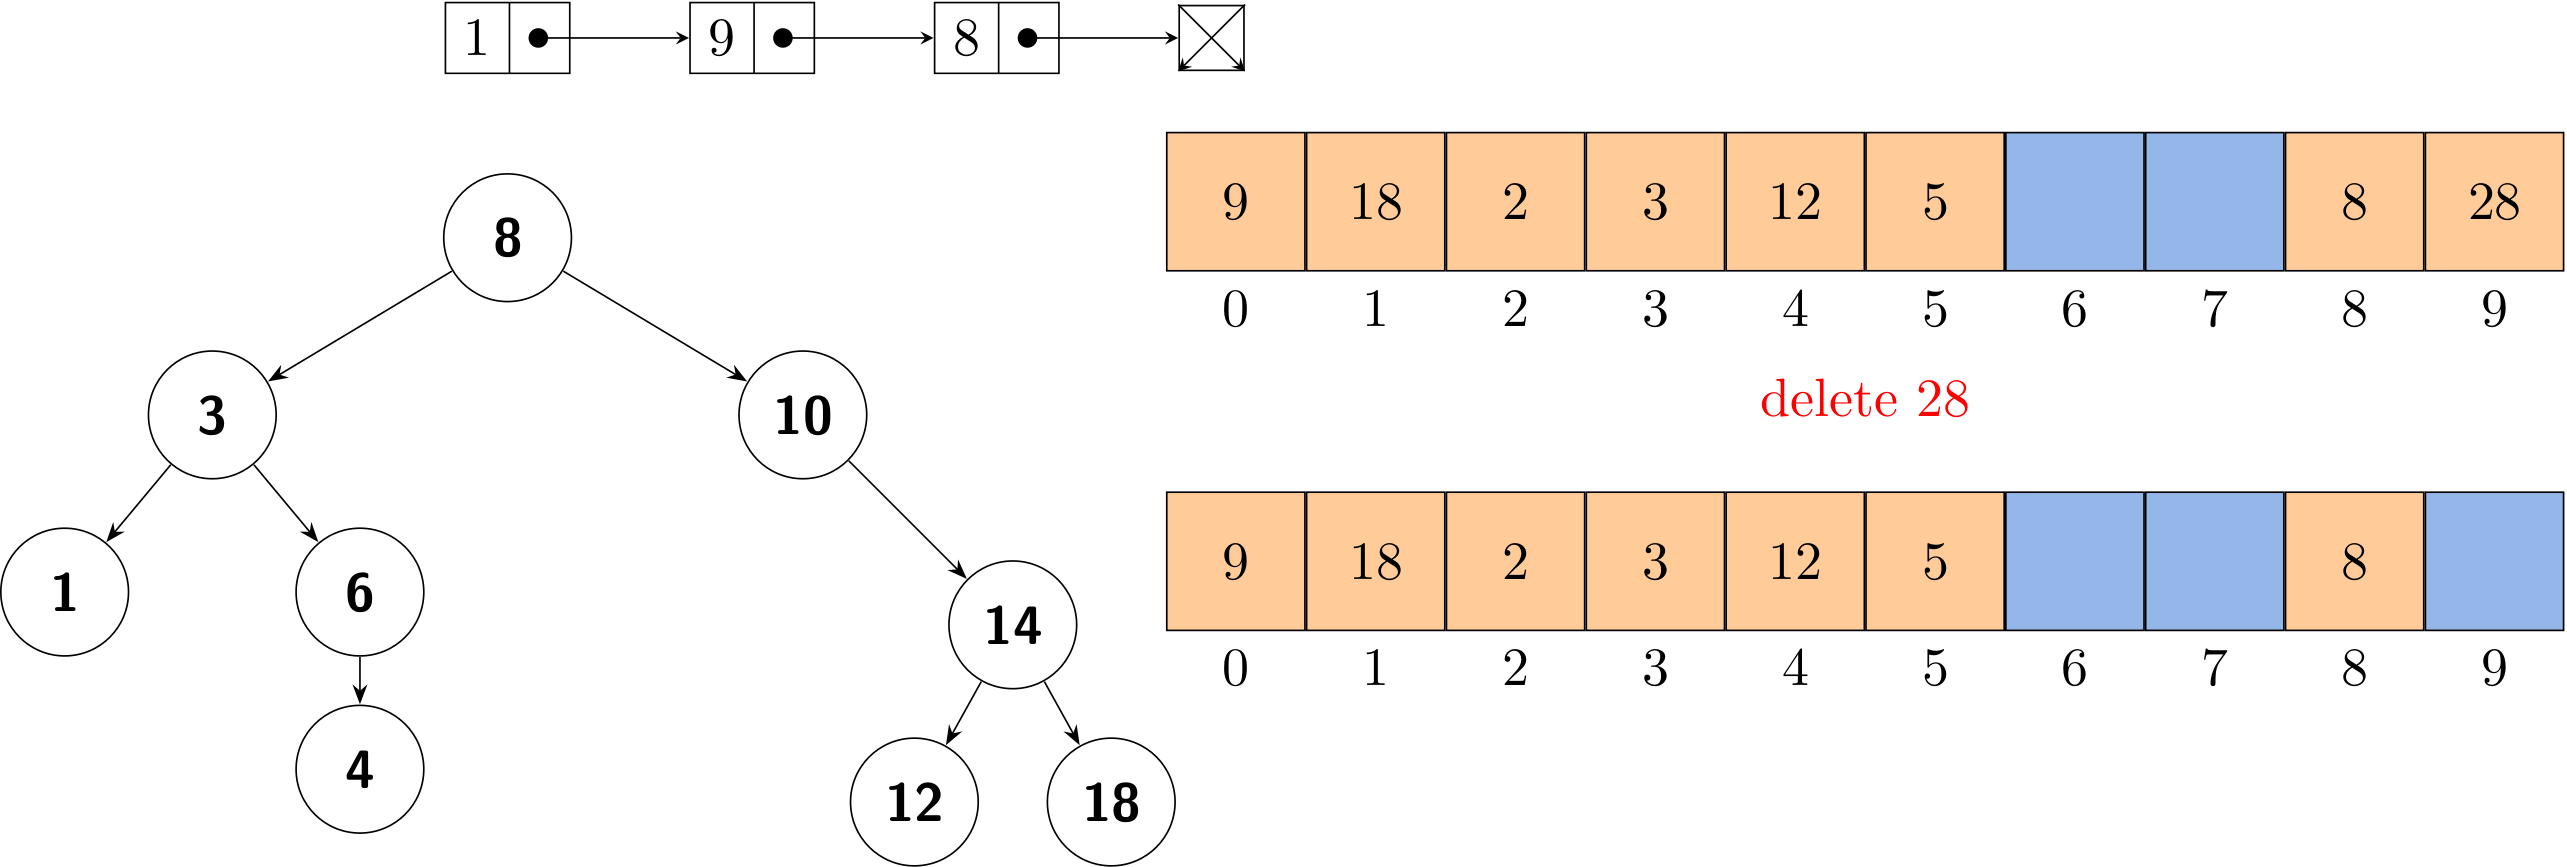
\includegraphics[height=0.7\paperheight]{cover}
    % \end{picture}    
    % }}
\usebackgroundtemplate{
  \tikz[overlay,remember picture] 
  \node[opacity=0.3, at=(current page.south east),anchor=south east, yshift=2cm,xshift=4cm] {
    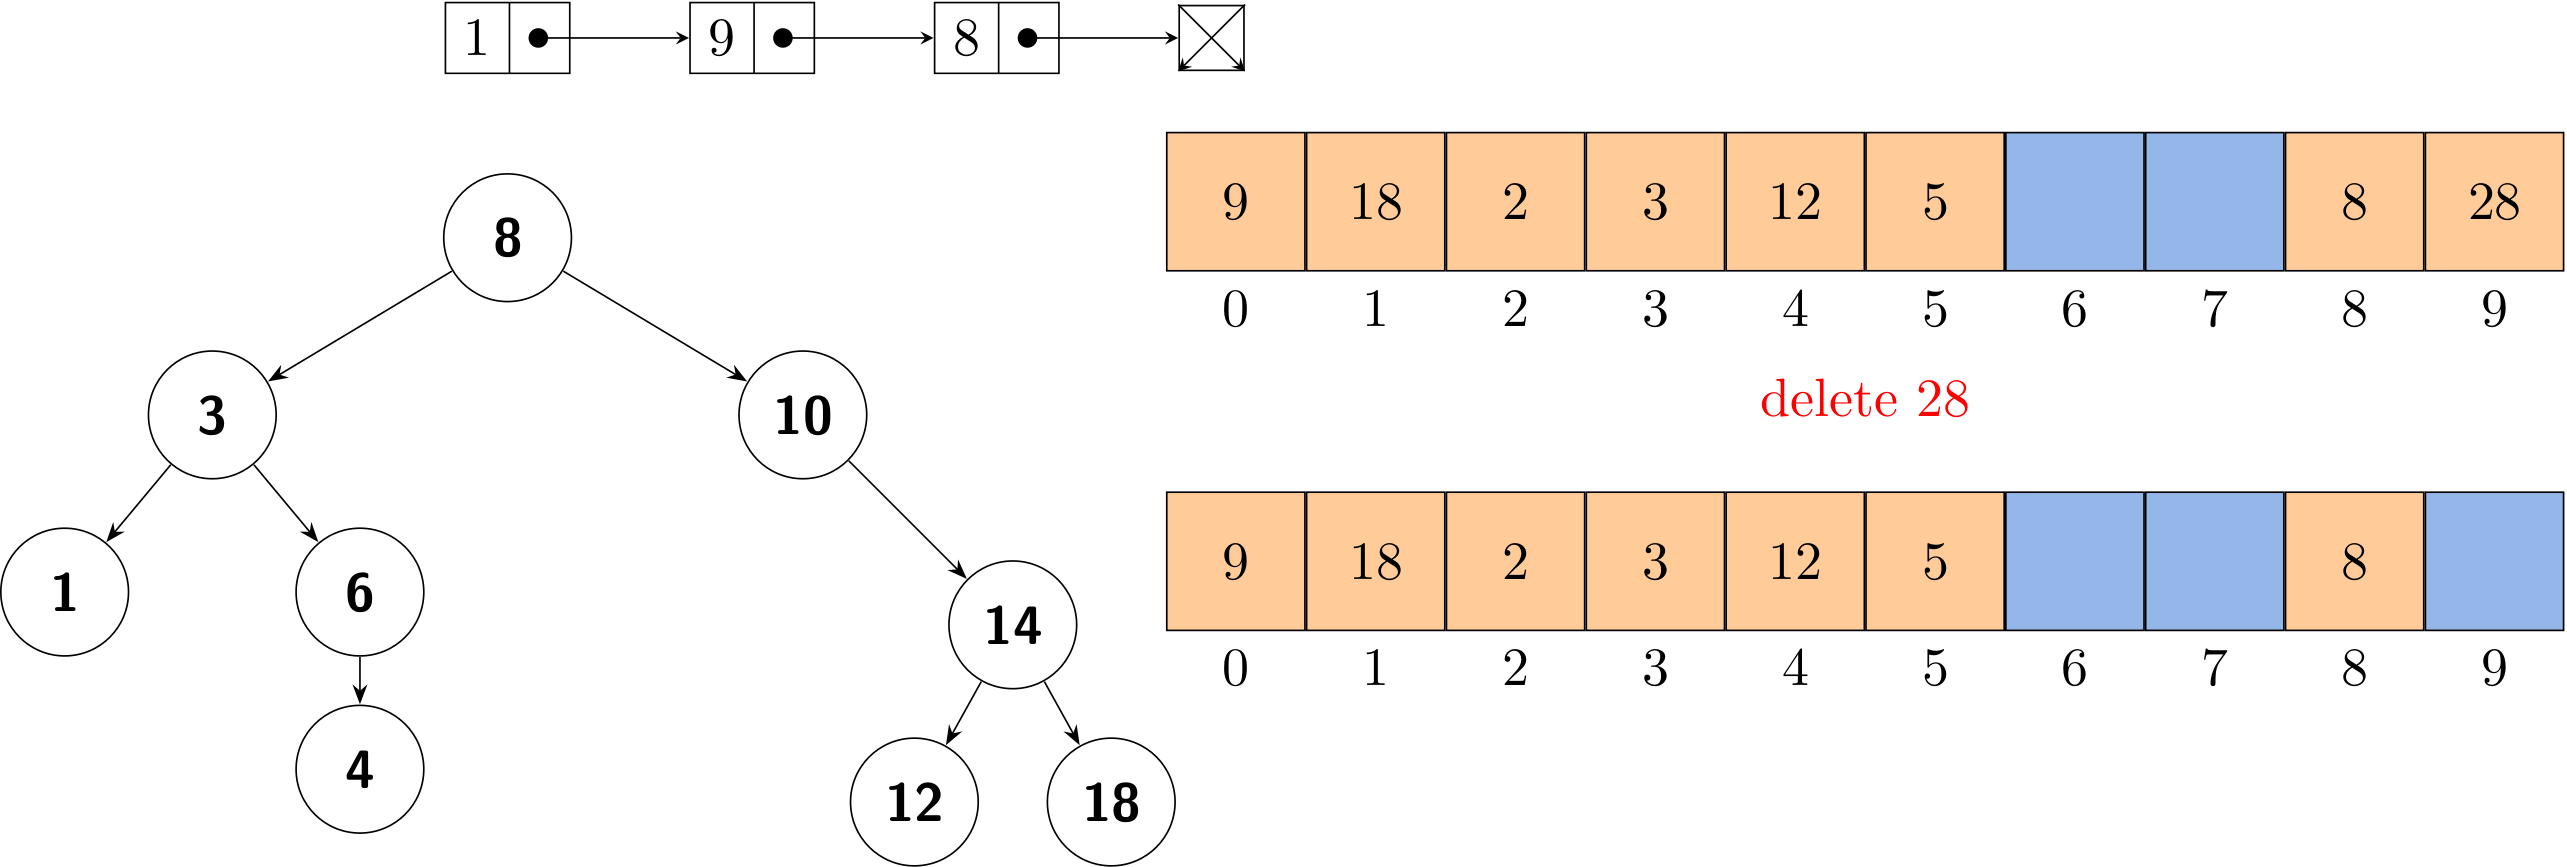
\includegraphics[height=0.6\paperheight]{cover}};
}
    \begin{frame}
        \section{\textcolor{darkmidnightblue}{2. Python Built-in Data Structures}}
    \end{frame}
}

\begin{frame}[fragile]
    \frametitle{2.1 List}
    Python's \alert{list} resembles Java's \emph{ArrayList}, representing a resizable array of items.

    \begin{minted}[bgcolor=LightGray]{python}
num = [1, 9, 4, 2]        
num = ['1', 9, 'four', 2]
for i in a:
    print(i)
squares = [x**2 for x in range(10)]
print(3 in num) # False
    \end{minted}    
\end{frame}

\begin{frame}[fragile]
    \begin{minted}[bgcolor=LightGray]{python}
print(num[0])
print(num[0:2])
print(num[:])
print(num[-1])
print(num[2:-1])    
    \end{minted}

\begin{exampleblock}{Question 1}
    How to get the size of a list in Python?
\end{exampleblock}

\begin{exampleblock}{Question 2}
How to get the last element of a list in Python?
\end{exampleblock}

\end{frame}

\begin{frame}
You are required to know and practice at least those methods:
\begin{enumerate}
    \item append()
    \item extend()
    \item insert()
    \item remove()
    \item pop()
    \item clear()
    \item sort()
    \item reverse()
\end{enumerate}    

\end{frame}

\begin{frame}[fragile]
    \frametitle{2.2 Set and Dict}
Python's \alert{set} resembles Java's \emph{HashSet}, representing an unordered collection of items without duplication.
\begin{minted}[bgcolor=LightGray]{python}
words = {'hello', 'world', 'hello'}
print(len(words))    
\end{minted}
\pause
Python's \alert{dict} resembles Java's \emph{HashMap}, representing a collection of key-value pairs.
\begin{minted}[bgcolor=LightGray]{python}
cart = {'7801': 3, '9902': 1}
print(cart['7801'])    
\end{minted}
\end{frame}

\begin{frame}[fragile]
    \begin{minted}[bgcolor=LightGray]{python}
empty_set = set()

empty_dict = {}
empty_dict2 = dict()

# When the keys are simple strings
words = dict(hello=2, world=1)
    \end{minted}
    
\pause
{\large \faIcon{lightbulb}} To prepare yourself for programming in Python, please read \href{https://docs.python.org/3/tutorial/datastructures.html}{5. Data Structures} thoroughly.
\end{frame}


\section{\textcolor{darkmidnightblue}{3. Why To Learn Data Structures?}}

\begin{frame}[fragile]
\begin{minted}[bgcolor=LightGray]{python}
books1 = ['Gone with the wind', 'Data structures']
books2 = {'Gone with the wind', 'Data structures'}
\end{minted}

Suppose there are $10^6$ books, which data structure shall we choose?

\pause

\begin{block}{Reasons}
    \begin{enumerate}
        \item Understanding how a data structure and algorithm work behind the scenes is necessary when choosing an appropriate one.
        \item Sometimes you should be a creator, not just a user.
    \end{enumerate}
\end{block}
\end{frame}

\begin{frame}
    \frametitle{Feynman: the way of learning}
    \begin{columns}
        \column{0.15\textwidth}
        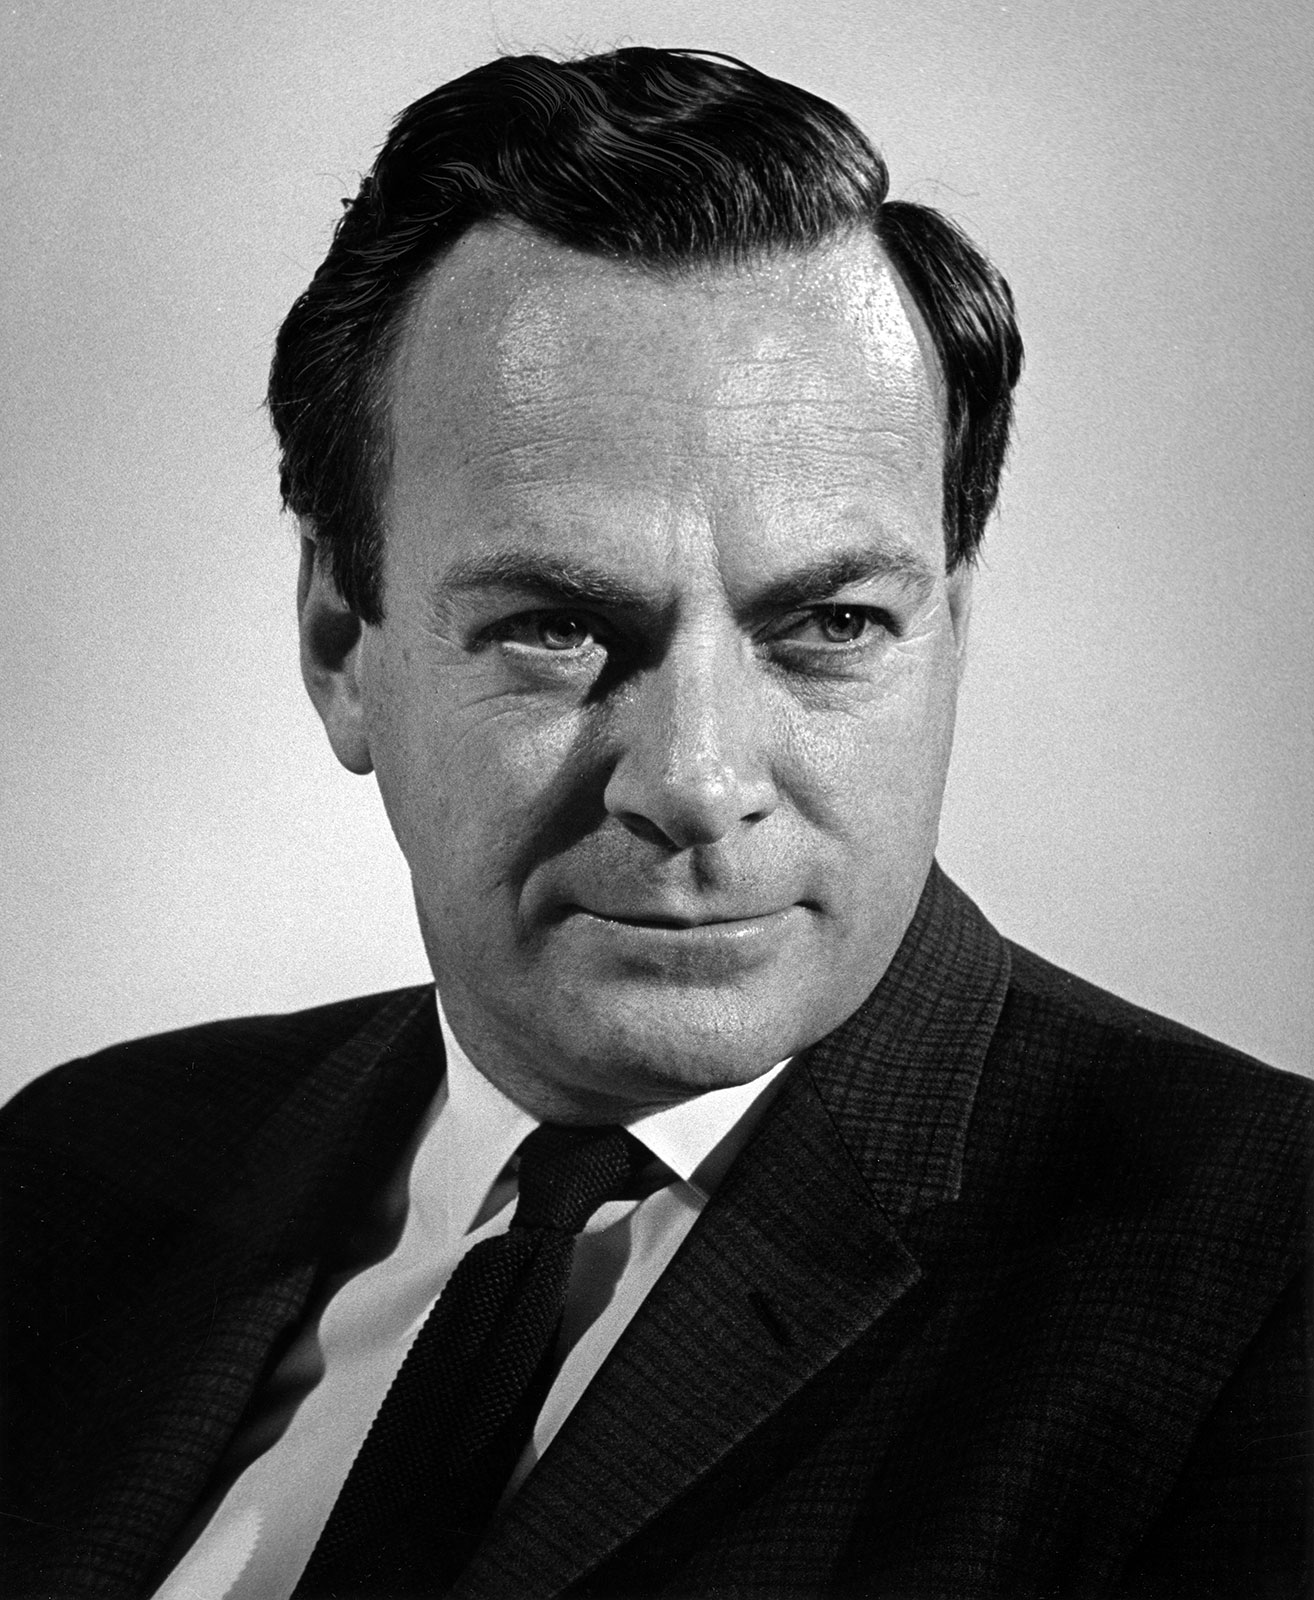
\includegraphics[height=0.5\paperheight]{week0/feynman}
        \column{0.85\textwidth}
        \begin{quote}
        ``See that bird?" he says. ``Well, in Italian, it's a Chutto Lapittida. In Chinese, it's a Chung-long-tah, and in Japanese, it's a Katano Tekeda. You can know the name of that bird in all the languages of the world, but when you're finished, you'll know absolutely nothing whatever about the bird." 
            (\textbf{I learned very early the difference between knowing the name of something and knowing something.})               
        \end{quote} 
    \end{columns}

\end{frame}


\begin{frame}
    \section{\textcolor{darkmidnightblue}{This Week's Task}}
\begin{itemize}
    \item Set up the developing environment (see more at Appendix)
    \item Practice \emph{list/set/map}.
\end{itemize}
\end{frame}
\end{document}